\chapter{Results}\label{chap:results}

In this chapter, primarily in the graphics, the implemented version is denoted
as `RUST', and the original Python implementation as `ICE'. This is done
consistently as a compromise to avoid confusion regarding two differently
colored `ICE' columns and too long identifiers. It should be clear that `RUST'
is not representative for the language, but only for this particular
implementation, also implementing ICE, not to confused with `ICE', the Python
implementation.

\section{Server Specification}\label{sec:specs}

See \tabref{tab:specs} for the specification of the test server.

\begin{table}[ht]
    \ra{1.3}
    \begin{tabular}{@{}lr@{}}
        \textbf{Virtual Server Specification} & \\
        \midrule
        Available Cores / Threads & 16 / 32 \\
        Working Memory (RAM) & 120 GByte \\ \\
        \textbf{Processor Specification} & \\
        \midrule
        Processor & Intel® Xeon® E5-2630V4\footnotemark \\
        Number of Cores/Threads & 10 / 20 \\
        Base/Turbo frequency & 2.2 GHz / 3.1 GHz \\
    \end{tabular}
    \caption[Server Specification]
    {\textbf{Server Specification.} \\
    For reproducibility, here are technical details about the hardware the
    following tests were run on.}
    \label{tab:specs}
\end{table}

\footnotetext{\url{https://ark.intel.com/content/www/us/en/ark/products/92981/intel-xeon-processor-e5-2630-v4-25m-cache-2-20-ghz.html}, accessed 2019-06-26}


\newpage
\section{Data for Testing}\label{sec:data}

\begin{table}[ht]
    \ra{1.3}
    \begin{tabular}{@{}lcr@{}}
        % \textbf{Matrix Details} & & & \\
        \textbf{Name}       & 25kb\_raw.h5  & 50kb\_raw.h5  \\
        \midrule
        Filesize            & 1.1 GByte     & 732 MByte     \\
        Size                & 123'841       & 61'928        \\
        Bin length          & 25'000        & 50'000        \\
        Non-zero elements   & 1'530'533'003 & 1'053'216'825 \\
    \end{tabular}
    \caption[Test Data]
    {\textbf{Test Data overview}.

    A third matrix, with a bin length of 10'000 was available, for which the
    existing working memory was not sufficient.} \label{tab:testdata}
\end{table}

% \begin{verbatim}
% # Matrix information file. Created with HiCExplorer's hicInfo version 3.0
% File:   matrix.h5
% Size:   309,581
% Bin_length:     10000
% Sum of matrix:  2416588411.2530212
% Chromosomes:    1, 2, 3, 4, 5, 6, 7, 8, 9, 10, 11, 12, 13,
%                 14, 15, 16, 17, 18, 19, 20, 21, 22, X, Y, MT
% Non-zero elements:      2,111,867,476
% Minimum (non zero):     0.008667398294551536
% Maximum:        139544.65657933566
% NaN bins:       25948

% The sizes of the matrices for reference (biggest to smallest):
% # Matrix information file. Created with HiCExplorer's hicInfo version 3.0
% File:   25kb_raw.h5
% Size:   123,841
% Bin_length:     25000
% Sum of matrix:  2378265786.0
% Chromosomes:    1, 2, 3, 4, 5, 6, 7, 8, 9, 10, 11, 12, 13,
%                 14, 15, 16, 17, 18, 19, 20, 21, 22, X, Y, MT
% Non-zero elements:      1,530,533,003
% Minimum (non zero):     1
% Maximum:        320932
% NaN bins:       9290

% # Matrix information file. Created with HiCExplorer's hicInfo version 3.0
% File:   50kb_raw.h5
% Size:   61,928
% Bin_length:     50000
% Sum of matrix:  2333794628.0
% Chromosomes:    1, 2, 3, 4, 5, 6, 7, 8, 9, 10, 11, 12, 13,
%                 14, 15, 16, 17, 18, 19, 20, 21, 22, X, Y, MT
% Non-zero elements:      1,053,216,825
% Minimum (non zero):     1
% Maximum:        320932
% NaN bins:       4514

% # Matrix information file. Created with HiCExplorer's hicInfo version 3.0
% File:   small_test_matrix.h5
% Size:   33,754
% Bin_length:     5000
% Sum of matrix:  35778.0
% Chromosomes:    chr2RHet, chr3RHet, chr2LHet, chr4, chrYHet, chr3L, chr2L,
%                 chrU, chrX, chrXHet, chr2R, chr3R, chrUextra, chrM, chr3LHet
% Non-zero elements:      69,213
% Minimum (non zero):     1
% Maximum:        8
% NaN bins:       0
% \end{verbatim}

Details about the different available matrices for further testing can be seen
in \tabref{tab:testdata}. These are matrices that have been shrunk in bin size
with \verb|hicMergeMatrixBins|, but the original data is from \cite{rao20143d}.






\begin{figure}[t]
    \begin{centering}
        % \subfloat[Some cool graphic]
        {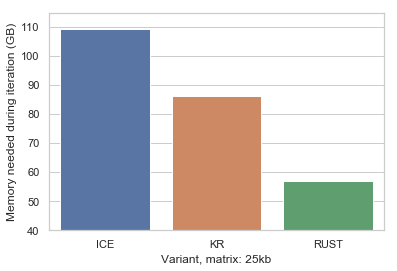
\includegraphics[scale=1]{figures/results/memiter_25}}
        \caption[Memory needs iterating 25kb]
        {\textbf{Memory needed during iteration} for correcting the 25kb matrix. Smaller is better.}
        \label{fig:memiter25}
\end{centering}
\end{figure}

\begin{figure}[t]
    \begin{centering}
        \subfloat[Available data]
        {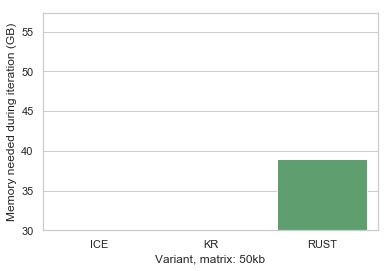
\includegraphics[scale=0.5]{figures/results/memiter_50}}
        \subfloat[Extrapolated data]
        {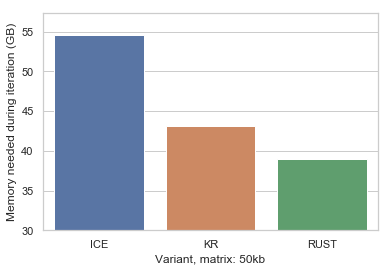
\includegraphics[scale=0.5]{figures/results/memiter_50_extra}}
        \caption[Memory needs iterating 50kb]
        {\textbf{Available and Extrapolated Data about Memory needed during
        iteration} of the 50kb matrix. Rust value is accurate, values for ICE
        and KR are not accurately available, but have been observed to be in
        the extrapolated areas. Smaller is better.}
        \label{fig:memiter50}
    \end{centering}
\end{figure}





\section{Memory Requirements}\label{sec:memory}

The memory requirements for these three algorithms are, or at least should be,
equal during loading, as the exact same code is executed. During loading,
memory was seen to fluctuate considerably, and was measured going up over 85
GByte at times. Initial loading time is proportional to matrix size, and
includes pre-processing. Prior to correction, zero values, \verb|NaN|s and
outliers are removed from the data. This needs between five and eight minutes
respectively (see \figref{fig:loadtimes} for reference).


\newpage
\subsection{During Correction}\label{sec:itermem}

Memory needs, at least for the iterative correction, have cycles. These cycles
correspond to the in \secref{sec:ICE} described steps, as the additional bias
matrices are not needed at any point other than for the correction itself. This
might be different for the implementation itself however, as e.g. in the Rust
implementation the memory needed for temporary biases is initialized before the
first iteration and is freed only after the last iteration finished.

A comparison of the three implementations regarding memory requirements during
correction of the 25kb connection matrix can be seen in \figref{fig:memiter25}.
As can be clearly seen, even though the recent KR implementation needs less
memory than the original ICE implementation, the new ICE implementation in Rust
needs even less, about half the amount the pure Python implementation needs.
Note that these are only comparisons of memory needs during iteration, there is
a different amount of memory needed for pre-processing and post-processing.

As can be seen in \figref{fig:memiter50}a, no reliable data except for the Rust
implementation exists for memory needs during computing of the 50kb matrix. In
\figref{fig:memiter50}b there is an extrapolation based on the data for the
25kb matrix and observed data, These values should not be taken at face value,
but they should not be too far off the truth. Here, the advantage of Rust
diminishes. Parts of the memory are still used from the initial pre-processing,
and the provided matrix itself (to the regarding algorithm) was only a copy.
Directly after loading (but before starting iteration), the needed memory when
correcting the 50kb matrix was 12GByte.


\subsection{Maximum required memory}\label{sec:maxmem}


\begin{figure}[!htbp]
    \begin{centering}
        \subfloat[Maximum resident set size when correcting 50kb matrix]
        {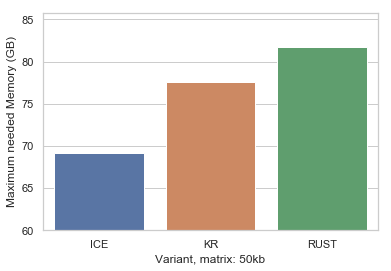
\includegraphics[scale=0.9]{figures/results/maxresident_50}} \\
        % \caption[Maximum needed Memory for 50kb]
        % {\textbf{Maximum needed Memory} when correcting the 50kb matrix.}
        \subfloat[Maximum resident set size when correcting 25kb matrix]
        {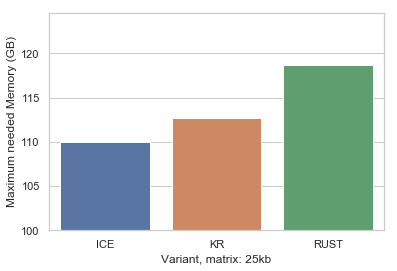
\includegraphics[scale=0.9]{figures/results/maxresident_25}}
        \caption[Maximum needed Memory]
        {\textbf{Maximum amount of needed Memory} when correcting 50kb and 25kb
        matrix. Smaller is better.}
        \label{fig:maxresident}
    \end{centering}
\end{figure}




Maximum required memory, or maximum resident set size, describes the highest
amount of memory needed at any point during execution. Maximum resident set size
is compared in \figref{fig:maxresident}.

After correction, the post-processing procedures differ. Both the Python and
C++ implementation return the corrected matrix as well as the correction
factors, while the Rust implementation is supposed to only return the
correction factors, as it does. This means that after returning the correction
factors, the corrected matrix from the rust part is not passed back, and a copy
of the original matrix is then corrected in Python again before saving the
corrected matrix.

When loading the matrix in the beginning, a considerable amount of working
memory is needed. However, the highest needs of memory are, at least for KR and
the RUST version, happening after the correction, when the corrected values are
set, the correction factors added and then saved. This might be due to
duplicate artifacts in memory, needing to be in memory in both Python and
the other language, while in the python version memory needs are considerably
lower during this process.

In Rust, indices are of type \verb|usize|, which size is platform-dependent. In
the case of the test server (more details in \secref{sec:specs} and
\tabref{tab:specs}) this is the size of a \verb|int64|, whereas coming from
Python (and thus most likely in C++) it is only a \verb|int32|. Indices are a
considerable amount of memory in the case of a CSRMatrix, as there are more
indices than there are actual elements in the matrix, and the elements are only
of type \verb|float32|.

It is unclear if the RUST implementation (or the post-processing, since it is
different) would use more memory if available, as the needed memory was
supremely close to the actually available one. It is also unclear, if this
implementation would use less if less was available. The required memory could
most likely be reduced by returning the corrected matrix as well, or directly
correcting the original matrix within the memory from Python. This has been
deemed possible, as the CSRMatrix structure is build on top of \verb|numpy|
ndarrays implementation, with \verb|numpy| having a well documented C-API.





\subsection{Load times}\label{sec:loadtime}


\begin{figure}[!htbp]
    \begin{centering}
        \subfloat[Loading time in minutes for 25kb matrix]
        {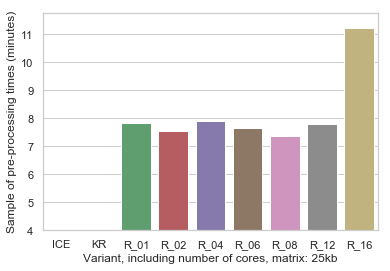
\includegraphics[scale=0.9]{figures/results/loadtimes_25}} \\
        % \caption[Correction time of 25kb]
        % {\textbf{Runtime in minutes} for correcting the 25kb matrix.}
        \subfloat[Loading time in minutes for 50kb matrix]
        {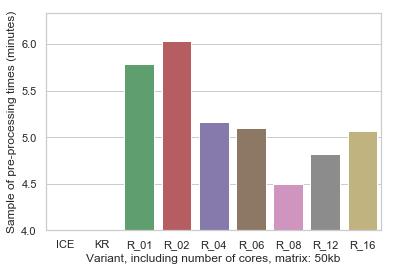
\includegraphics[scale=0.9]{figures/results/loadtimes_50}}
        \caption[Matrix loading times]
        {\textbf{Matrix loading times} for the different matrix sizes. Even though
        the operations are the same during pre-processing, actual times fluctuated.
        No data is available for ICE and KR variants, however as the pre-processing
        is the same, their values can be thought to be in the same range as the
        others. Equal is better.}
    \label{fig:loadtimes}
    \end{centering}
\end{figure}




Loading includes pre-processing the to-be corrected matrices. Pre-processing
steps include removal of zero-values, \verb|NaN|s from the dataset and
heavy outliers, as they would affect correction. However, even though the same
steps were performed in all cases, load times had significant outliers, as can
be seen in \figref{fig:loadtimes}. Here, loading times from separate runs are
shown. The runs differ in that they were run in different configurations, which
start to differ after loading, as explained in more detail in
\secref{sec:multicore}. However as there is no difference up to this point,
they can very well be compared. Considering that there should no difference, it
is shocking to see that significant differences between loading times exist.

In the case of \figref{fig:loadtimes}a, most loading times are within half a
minute of each other, which could still be called deterministic considering the
size of the matrix and the amount of data written back and forth. The big jump
as seen in variant R\_16 however, should not be possible. Considering an
average time of around 7.5 minutes, 11.2 minutes are close to 50\% more than
that (49.4\%) ! This can only be described by the conditions of the virtual
server varying based on usage from other users, for which there is no data
available, except for deviations in this data, without knowledge what the
actual values would have been.

Loading times in \figref{fig:loadtimes}b do not differ by proportions as high,
but the clearly visible disparity is not something favorable.
% longest seen from the shortest is 33\% longer\footnote{(6 - 4.5) / 4.5
% = 33\%}, and the shortest is 25\% shorter when compared to the
% longest\footnote{(6 - 4.5) / 6 = 25\%}.


\subsection{Comparing Memory needs}\label{sec:compmemory}

\begin{table}[!htbp]
    \begin{tabular}{lrrr}
        \textbf{Overall memory comparison} & ICE & KR & RUST \\
        \midrule
        During iteration (50kb) &   54.6 & 43.1 & \textbf{39}   \\
        Maximum          (50kb) &   \textbf{69.2} & 77.6 & 81.7 \\
        During iteration (25kb) &   110 & 86 & \textbf{57}  \\
        Maximum          (25kb) &   \textbf{110} & 112.7 & 118.6 \\
    \end{tabular}
    \caption[Memory needs comparison]
    {\textbf{Overall comparison} between required memory for different
    situations. The ICE values for Maximum resident values are not considered,
    as they are probably wrong for some reason. See \secref{sec:maxmem} for
    details.}
    \label{tab:compmem}
\end{table}

As can be seen in \tabref{tab:compmem}, regarding memory usage each of the
algorithms has some advantage and another disadvantage. If working memory is a
critical resource, the question as to which is more critical, long-term lower
usage, or lower spike usage, becomes decisive for the selection of the
algorithm.




\section{Runtime length}\label{sec:runtime}


\begin{figure}[!htbp]
    \begin{centering}
        \subfloat[Runtime in minutes for correcting 25kb Matrix]
        {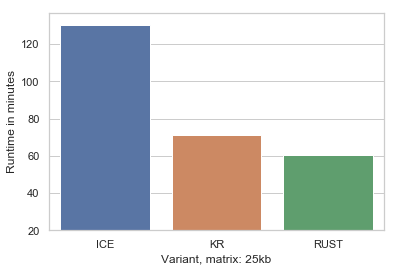
\includegraphics[scale=0.9]{figures/results/runtime_25}} \\
        % \caption[Correction time of 25kb]
        % {\textbf{Runtime in minutes} for correcting the 25kb matrix.}
        \subfloat[Runtime in minutes for correcting 50kb Matrix]
        {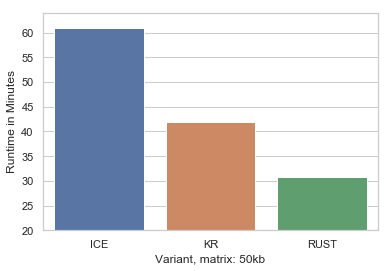
\includegraphics[scale=0.9]{figures/results/runtime_50}}
        \caption[Algorithm Runtimes]
        {\textbf{Algorithm Runtimes} for correcting the different matrices. It
        remains an open question why the difference between KR and RUST stays the
        same, even though both ICE and RUST double their computation time. Smaller
        is better.}
        \label{fig:runtime}
    \end{centering}
\end{figure}



In \figref{fig:runtime} a comparison of runtimes can be seen. The original
implementation in Python is taking the longest by a considerable amount, with
the implementation in Rust needing about half the time in both situations, less
than KR which is at only a third for 50kb. The difference itself, which is
about ten minutes, is roughly the same for both matrices though. In both cases
the difference is around ten minutes, whereas it is proportionally more when
the total runtime is only four times that amount versus ten minutes being only
a seventh of the total runtime, \figref{fig:runtime}b and \figref{fig:runtime}a
respectively.

An open question remains as to why this difference is roughly the same, even
though the python implementation needs about twice as much time, as does the
Rust one. It might be that the KR implementation is faster for considerably
bigger matrices. Testing this was not possible as the memory of the provided
virtual machine (see \secref{sec:specs} and \secref{sec:maxmem} for details)
did not allow loading of bigger matrices, and repeatedly failed trying to do
so.



\section{Multicore benefits}\label{sec:multicore}


\begin{figure}[!tbp]
\begin{centering}
    % \subfloat[Runtime in minutes for correcting 50kb Matrix]
    {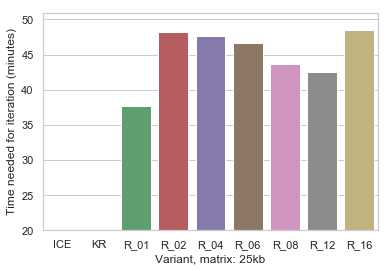
\includegraphics[scale=0.8]{figures/results/compute_multi_25}}
    \caption[Multicore comparison]
    {\textbf{Algorithm Runtimes} for correcting the different matrices. Smaller is better.}
    \label{fig:computetime25}
\end{centering}
\end{figure}




As can be seen in \secref{demo:par}, turning a single-core Rust program into
a multi-core program is not particularly difficult. Taking a look at
\figref{fig:computetime25}, the advantage of using multiple cores is everything
but apparent, in fact it is even slower than not using it. There are multiple
reasons for this. First, most of the parallelized operations are considerably
small, sometimes just slightly more complex than a list summation. In the case
of parallelizing list summations as well, total runtime becomes similar to the
original ICE implementation, as there are several summations for each
iteration. Even though the operations themselves are rather small, the overhead
for how to distribute them is still added, even in the case of using only one
core. This overhead is spreaded across several cores as well, but even using 12
cores is not sufficient for amortizing the additional overhead. The scheduler
of \verb|rayon|, the used library for this, is a work-stealing scheduler,
meaning that initially every thread in the thread pool gets a roughly equal
amount, and as soon as one core is done earlier than the others, its stealing
work from other cores. Initially all work is distributed over the available
threads in chunks. This initial distribution makes up a significant amount of
overhead. In the case of 16 Threads (and above in cases tested), the main
overhead is coming from too many threads having finished earlier and stealing
work from each other.

Even though the current version does support parallelization, it does not
provide benefits. They might only visualize for even bigger matrices, where the
amount of needed work amortizes the initial overhead better. Additionally,
there is more potential for combining operations for parallelization. For some,
this is clearly not possible, but for several it would be possible to combine
them, reducing the overhead for parallelization at one point, and parallelizing
heavier operations instead.


\begin{figure}[!htbp]
    \begin{centering}
        \subfloat[Memory needed during iteration when correcting 25kb matrix]
        {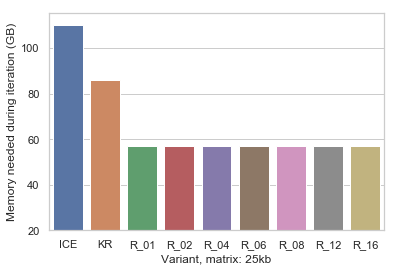
\includegraphics[scale=0.5]{figures/results/memiter_multi_25}}
        \subfloat[Maximum resident set size when correcting 25kb matrix]
        {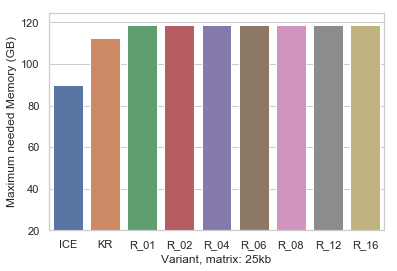
\includegraphics[scale=0.5]{figures/results/maxresident_multi_25}}
        \caption[Multicore Memory comparison]
        {\textbf{Multicore Memory needs} for correcting the 25kb matrix. Memory
        needs stay the same in all versions. Based on the numbers, there is no
        difference between the single-core version and any multi-core version
        regarding memeory usage.}
        \label{fig:memmulti}
    \end{centering}
\end{figure}


\begin{figure}[!htbp]
    \begin{centering}
        % \subfloat[subfloat-text]
        {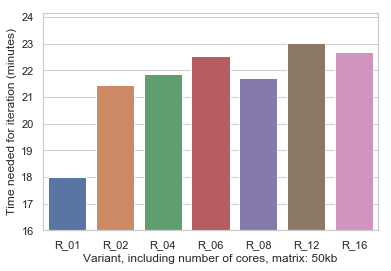
\includegraphics[scale=0.8]{figures/results/runtime_multi_50}}
        \caption[Multi-core computation time comparison]
        {\textbf{Multi-core computation time comparison} for 50kb matrix. These are
        pure computing times, excluding both pre- and post-processing. No numbers
        for ICE and KR are available. Smaller is better.}
        \label{fig:mrun50}
    \end{centering}
\end{figure}


However, as can be seen in \figref{fig:memmulti}, memory is not negatively
affected in any way when parallelizing. Regarding memory, the same holds true for
the 50kb matrix. Pure computation times for the 50kb matrix as seen in
\figref{fig:mrun50} do not seem to offer a clear trend regarding the usage of
multiple cores.


\paragraph{Conclusion:} Using multiple cores for this implementation does not
provide any benefit, however it does have significant downsides other than
longer runtime. The algorithm may be rewritten to allow better multicore usage.



\section{Output}

\begin{figure}[!htbp]
    \begin{centering}
        \subfloat[original values]{
            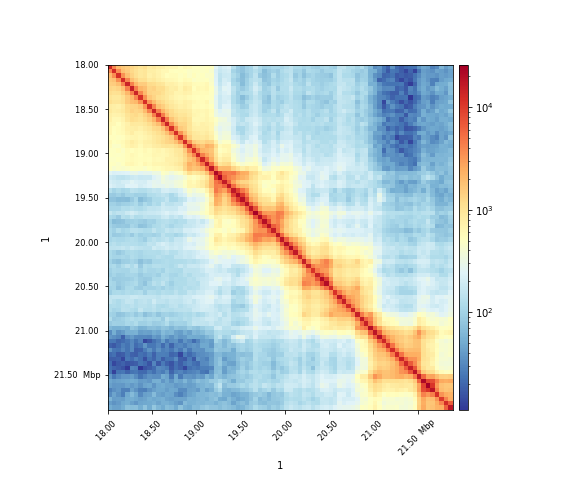
\includegraphics[scale=0.4]{figures/results/c_50kb}}
        \subfloat[RUST]{
            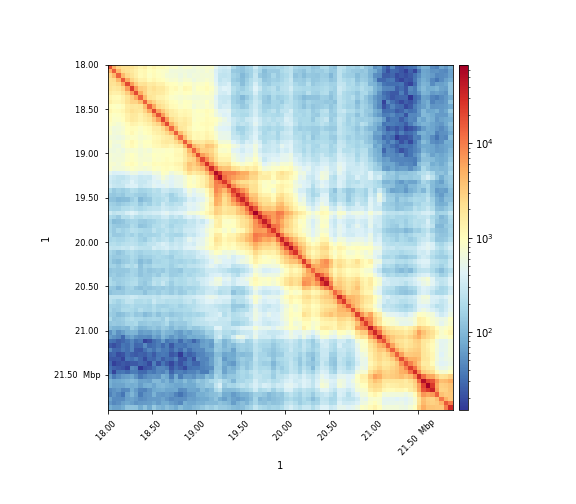
\includegraphics[scale=0.4]{figures/results/c_rust_50kb}} \\
        \subfloat[ICE]{
            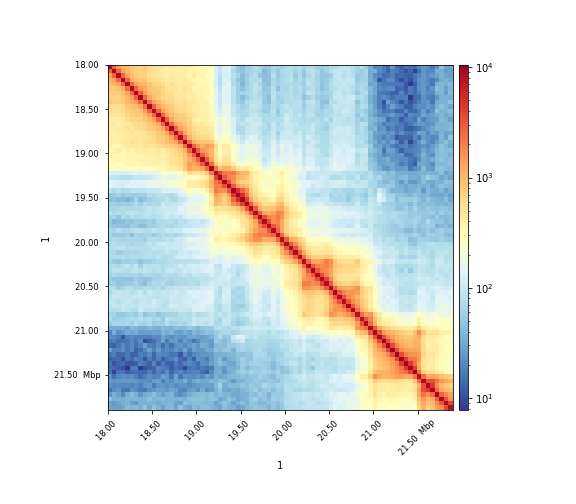
\includegraphics[scale=0.4]{figures/results/c_ice_50kb}}
        \subfloat[KR]{
            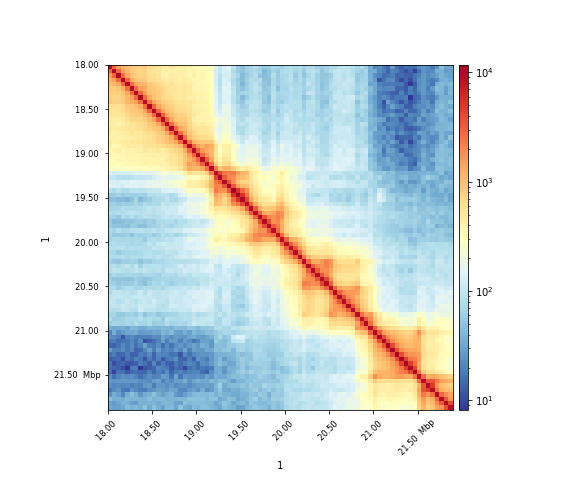
\includegraphics[scale=0.4]{figures/results/c_kr_50kb}}
        \caption[Plotting corrected matrices]
        {\textbf{Original and corrected matrices.} In \textbf{(b)} there appear to be
        higher maximum values, setting the cutoff lower creates pictures
        undistinguishable to those from ICE or KR.
        Images were created using hicPlotMatrix.
        }
        \label{fig:plotted}
    \end{centering}
\end{figure}


One essential point of a reimplementation is the correctness of of the output.
As can be seen in \figref{fig:plotted}, the output from both the original ICE
implementation and the KR version are pretty much the same. The output of the
RUST implementation is closer to the original values however. Due to time
constraints the differences between the output matrix in the Rust implementation
could not be further explored, but are likely due to different thresholds in
the implementation of the algorithm.





% using hicPlotMatrix -m <matrixname> --region 1:18000000-22000000 --log1p -o <outfile>.png

